\chapter{Implementacja}

Silnik kategoryzacyjny został zaimplementowany w języku C++, z użyciem środowiska Visual Studio w wersji 2010 Express, która jest podstawową wersją tego środowiska. Licencja na to oprogramowanie jest wydawana bezpłatnie, niezależnie od tego czy wykorzystujemy je do celów edukacyjnych czy komercyjnych. Posiada ograniczenie w dostępie do wtyczek, nie posiada możliwości zdalnego debugowania, analizy kodu oraz kompilowania do 64 bitowego kodu.

\section{Język C++ i Visual Studio}

Język C++ jest językiem programowania ogólnego przeznaczenia. Jest językiem wieloparadygmatowym, czyli umożliwia stosowanie różnych paradygmatów programowania: proceduralnego, obiektowego i generycznego. Został zaprojektowany przez Bjarne Stroustrupa jako rozszerzenie języka C i użyty po raz pierwszy w 1979 roku. Charakteryzuje się obiektowymi mechanizmami abstrakcji danych oraz silną statyczną kontrolą typów.

Początkowo do realizacji zadania miał zostać wykorzystany język Python, ze względu na bogactwo bibliotek do uczenia maszynowego oraz przetwarzania obrazów. Warto wspomnieć szczególnie o dwóch bibliotekach: scikit-learn oraz scikit-image, które pozwalają na rozwiązanie wielu problemów związanych z klasyfikacją obrazów, klastrowaniem lub ekstrakcją cech. Zdecydowano o użyciu języka C++ z dwóch powodów:

\begin{compactitem}
	\item \emph{szybkość działania} -- kod jest kompilowany do kodu maszynowego, natomiast Python jest językiem interpretowanym i przez to czas potrzebny na osiągnięcie podobnych wyników jest większy,
	\item \emph{silne typowanie} -- w przeciwieństwie do Pythona, język C++ jest silnie typowany, co w ocenie autora niniejszej pracy ma wpływ na zachowanie porządku w kodzie źródłowym.
\end{compactitem}

Microsoft Visual Studio jest zintegrowanym środowiskiem programistycznym rozwijanym przez firmę Microsoft. W skład pakietu wchodzą kompilatory kilku języków: C\#, J\#, Visual Basic, F\#, C++ oraz zintegrowany debugger, który działa na poziomie kodu źródłowego, jak i maszyny. Pierwsze wydanie pakietu pojawiło się w 1995 i obecnie najnowszą wersją jest wersja 12 z 2013 roku. 

Kompilator Visual C++ wchodzący w skład pakietu jest specjalną wersją kompilatora języka C++, dostosowana do systemu Windows. Z tego powodu zawiera wiele dedykowanych bibliotek dla tego systemu operacyjnego, które nie mają swoich odpowiednikach w systemach Linux, Unix lub Mac OS X. Dodatkowo Microsoft wydając ten kompilator stworzył swój własny standard języka, który do wersji Visual Studio 2013 nie był w pełni zgodny z ISO. Co za tym idzie, kod silnika powstały w wersji Visual Studio 2010 nie musi być zgodny z ISO. Na rys. \ref{fig:visual-studio-main-window} przedstawiono widok głównego okna środowiska Visual Studio 2010 Express.

\begin{figure}[h]
	\centering
	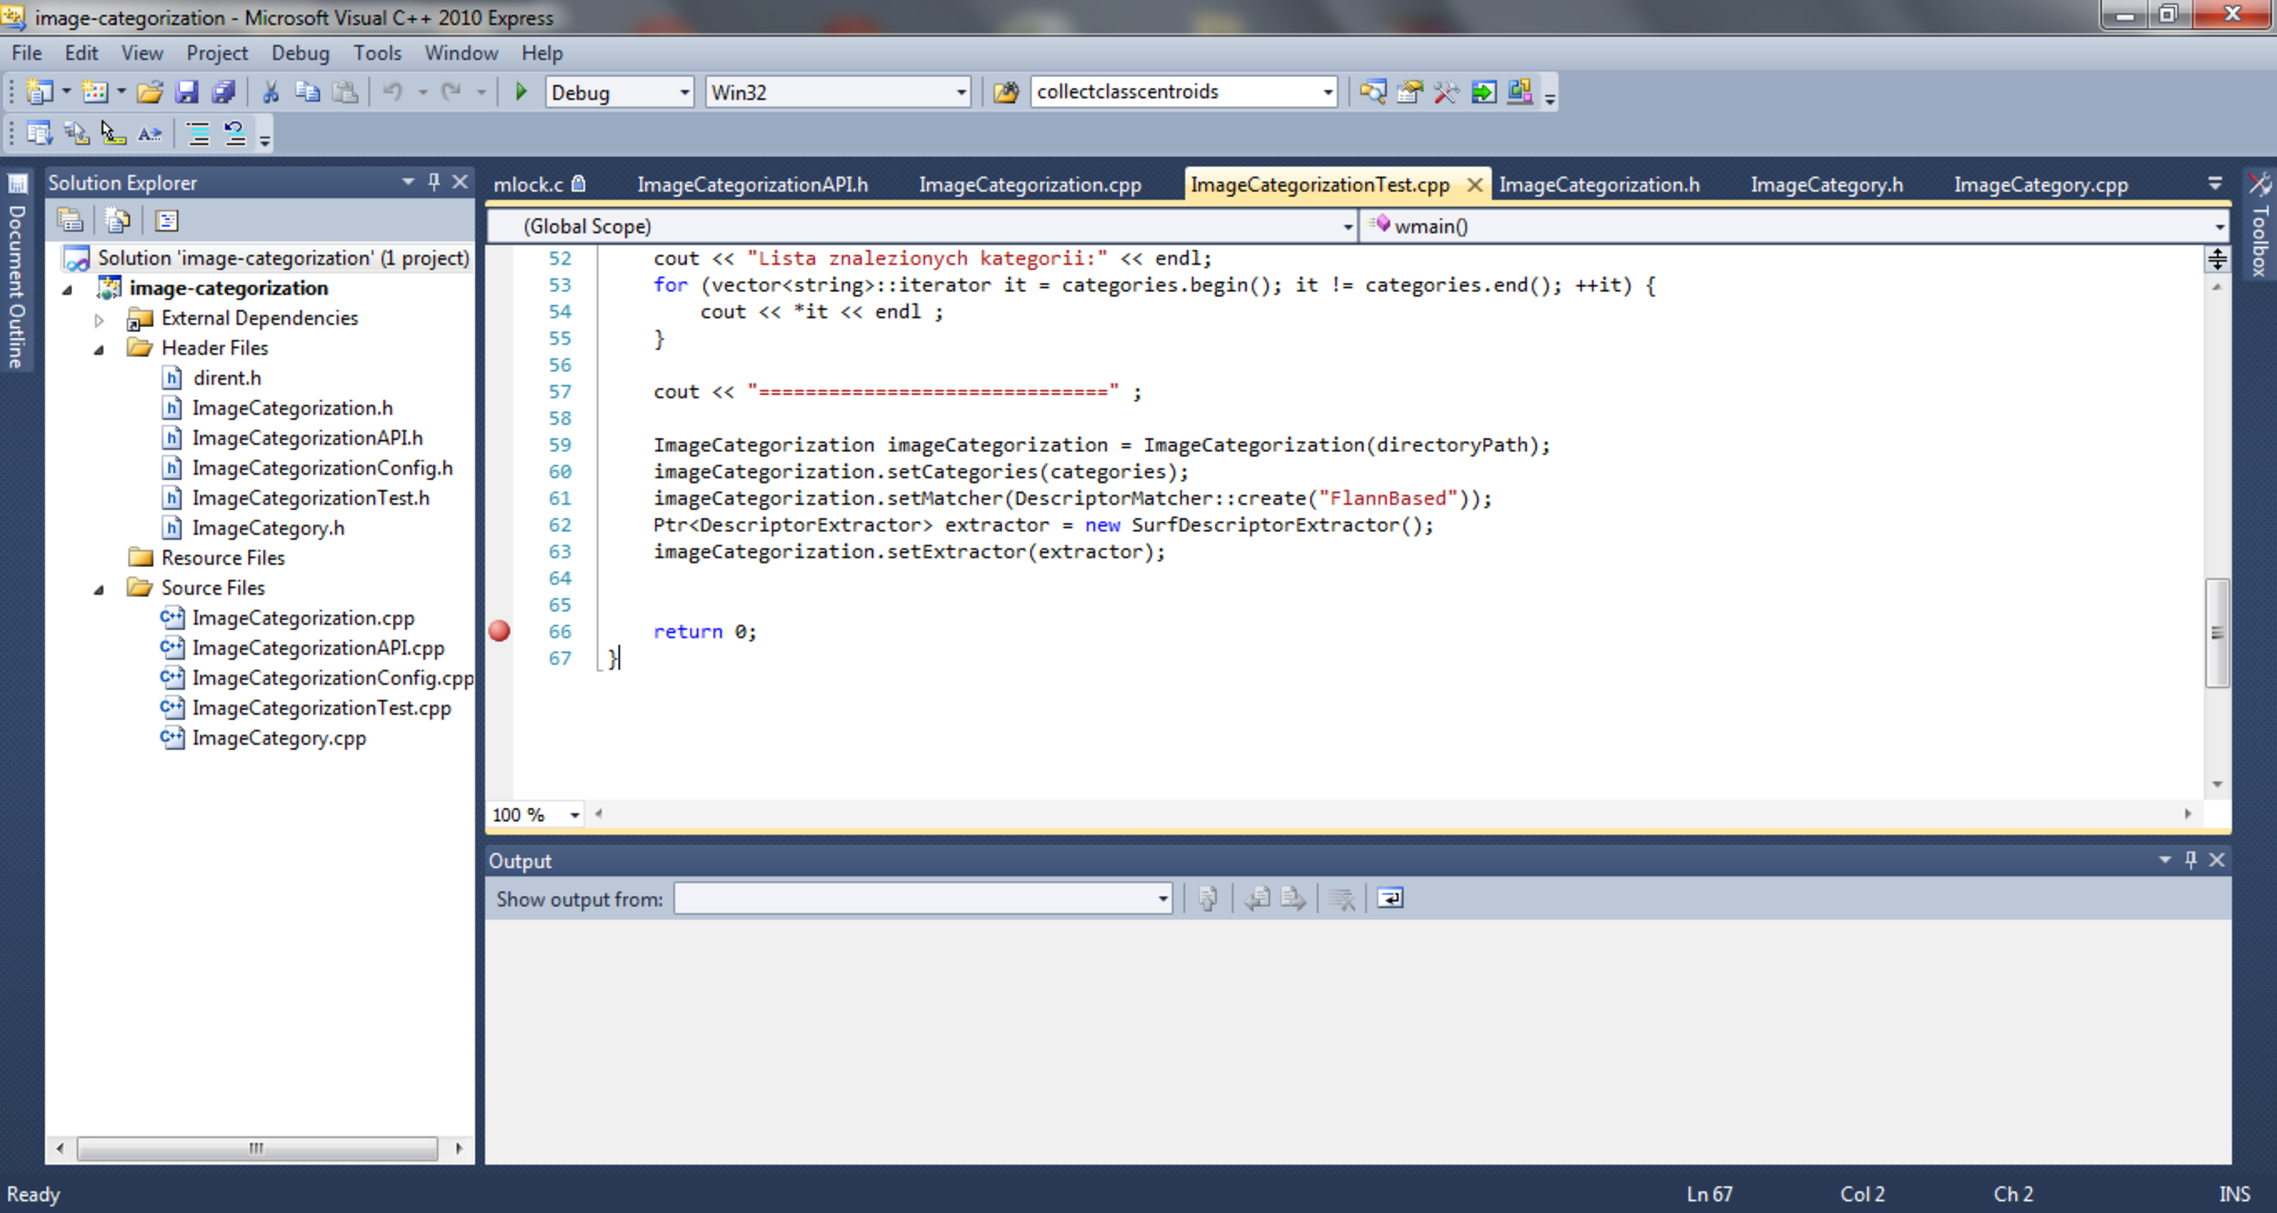
\includegraphics[scale=0.4]{graphics/03_implementacja/visual-studio-main-window.pdf}
	\caption{ Główne okno środowiska programistycznego Micsoroft Visual Studio 2010 Express }
	\label{fig:visual-studio-main-window}
\end{figure}

\section{OpenCV}

Do ekstrakcji cech oraz do klasyfikacji wykorzystano OpenCV. Jest to biblioteka do przetwarzania obrazów napisana w języku C, oparta na otwartym kodzie i zapoczątkowana przez firmę Intel. Charakteryzuje się wieloplatformowością, gdyż istnieją wersje na systemy operacyjne Windows, Mac OS X oraz Linux. Umożliwia ponadto, dzięki zastosowaniu odpowiednich nakładek, na tworzenie kodu w różnych językach programowania: C++, C\# oraz Python. Do realizacji zadania wykorzystano OpenCV w wersji 2.2.0.

\section{Architektura systemu}
Zaproponowany system do kategoryzacji obrazów wykorzystuje podejście \emph{Bag of Keypoints}\cite{CSURKA04}. Metoda ta opiera się na kwantyzacji wektorowej deskryptorów i odpowiada histogramowi przypadków występowania poszczególnych wzorców na obrazie. Metoda ta adaptuje podejście \emph{Bag of Words}, które było wcześniej używane do kategoryzacji tekstowej\cite{TONG00}, na potrzeby kategoryzacji obrazów. Do zalet tej metody należy zaliczyć prostotę, wydajność obliczeniową oraz niezależność od przekształceń afinicznych oraz oświetlenia.\cite{CSURKA04} Często metoda ta jest również nazywana metodą \emph{Bag of Words}\cite{TENG11} (tak samo jak w przypadku kategoryzacji tekstu) lub \emph{Bag of Visual Words}\cite{KESORN12}.

Na rys. \ref{fig:bag-of-keypoints} przedstawiono mechanizm działania metody \emph{Bag of Keypoints}. Do ekstrakcji punktów charakterystycznych użyto algorytmów SIFT oraz SURF, w celu określenia który z nich daje lepsze wyniki dla kategoryzacji zbioru testowego. Punkty charakterystyczne znalezione na różnych obrazach są następnie klastrowane w celu znalezienia zbioru podobnych do siebie fragmentów obrazów. W celu określenia, które fragmenty są do siebie podobne użyto biblioteki FLANN (\emph{Fast Approximate Nearest Neighbor Search}). Powstałe w ten sposób klastry często określa się jako słowa wizualne (\emph{ang. visual words}).

Następnie jako deskryptor obrazu używane są histogramy częstości występowania poszczególnych słów wizualnych. Jako klasyfikator została użyta maszyna wektorów nośnych (SVM).

\begin{figure}[h]
	\centering
	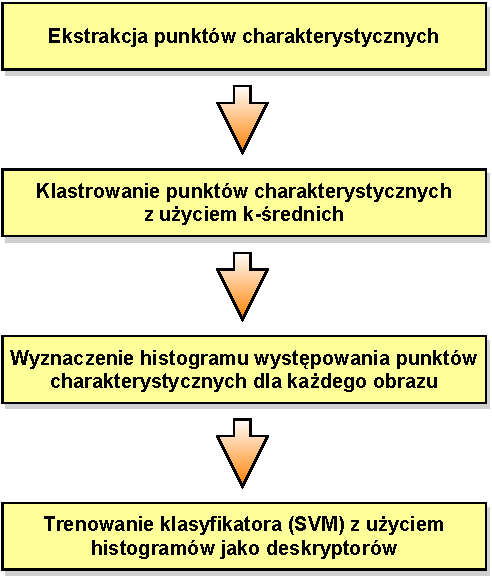
\includegraphics[scale=1.0]{graphics/03_implementacja/bag-of-keypoints.pdf}
	\caption{ Schemat działania metody \emph{Bag of Keypoints} }
	\label{fig:bag-of-keypoints}
\end{figure}

Projekt składa się z następujących klas:
\begin{compactitem}
	\item \emph{ImageCategorization} -- odpowiada za ekstrakcję cech oraz proces kategoryzacji, 
	\item \emph{ImageCategorizationAPI} -- udostępnia publiczne API pozwalające na tworzenie modelu kategoryzacyjnego, uczenie na podstawie przygotowanych zestawów przykładów, określanie kategorii wybranego obrazu,
	\item \emph{ImageCategorizationTest} -- umożliwia przeprowadzenie testowania skuteczności procesu kategoryzacji na podstawie przykładowych zestawów uczących i testowych.
\end{compactitem}

\section{Konfiguracja środowiska}
Aby uruchomić program w środowisku Windows, należy w pierwszej kolejności zainstalować Microsoft Visual Studio 2010 Express oraz OpenCV w wersji 2.2.0. Domyślnie biblioteka OpenCV instalowana jest w lokalizacji \emph{C:\textbackslash OpenCV2.2}. Przed uruchomieniem projektu wymagane jest wykonanie następujących kroków:
\begin{enumerate}
  \item Dodanie do zmiennej systemowej PATH lokalizacji biblioteki OpenCV. Można to zrobić w Panelu sterowania systemu Windows wchodząc do opcji "System" w Panelu sterowania, a następnie wybierając "Zaawansowane ustawienia systemu" i klikając na guzik "Zmienne Środowiskowe...". Następnie na liście "Zmienne systemowe" należy odnaleźć zmienną "Path" i kliknąć na "Edytuj...". W oknie edycji należy dopisać do końca listy \emph{C:\textbackslash OpenCV2.2} upewniając się, że poprzedni wpis został oddzielony za pomocą znaku ';' (rys. \ref{fig:ustawienia-path}).
  
	\begin{figure}[h]
		\centering
		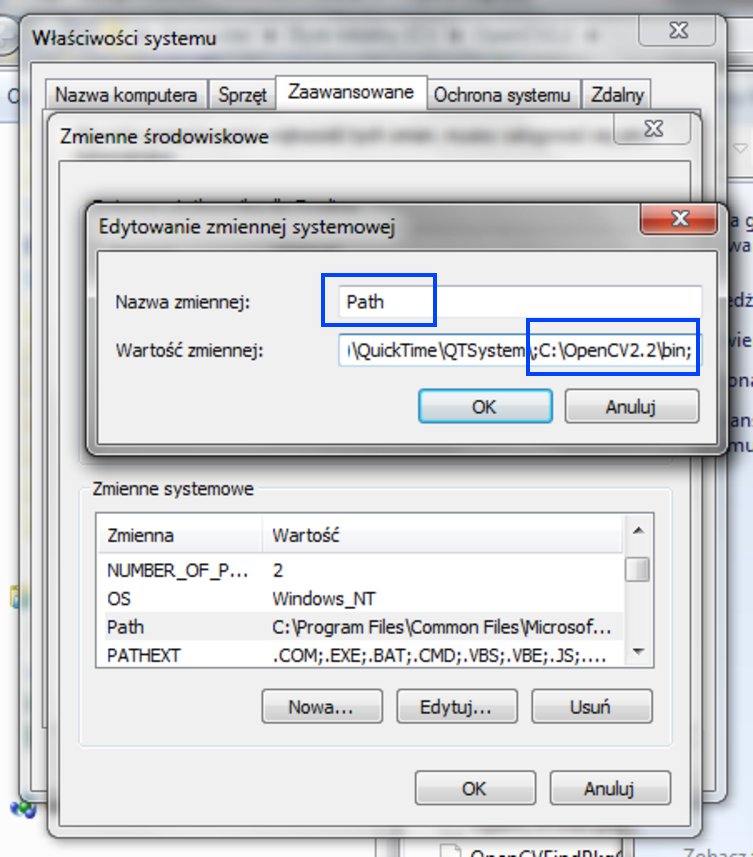
\includegraphics[scale=1.0]{graphics/03_implementacja/ustawienia-path.pdf}
		\caption{ Ustawienie zmiennej środowiskowej PATH w systemie Windows }
		\label{fig:ustawienia-path}
	\end{figure}
  
  \item Następnie należy otworzyć projekt w programie Visual C++ 2010 Express i przejść do ustawień projektu klikając prawym przyciskiem myszy na ikonę reprezentującą projekt w "Solution Explorer" i wybierając opcję "Properties".
  \item W zakładce "VC++ Directories" należy edytować "Include Directories" i dodać do listy katalogów lokalizacje \emph{C:\textbackslash OpenCV2.2\textbackslash include} oraz \emph{C:\textbackslash OpenCV2.2\textbackslash include\textbackslash opencv}, a następnie kliknąć na przycisk "OK" (rys. \ref{fig:ustawienia-include-dirs}).
  
	\begin{figure}[h]
		\centering
		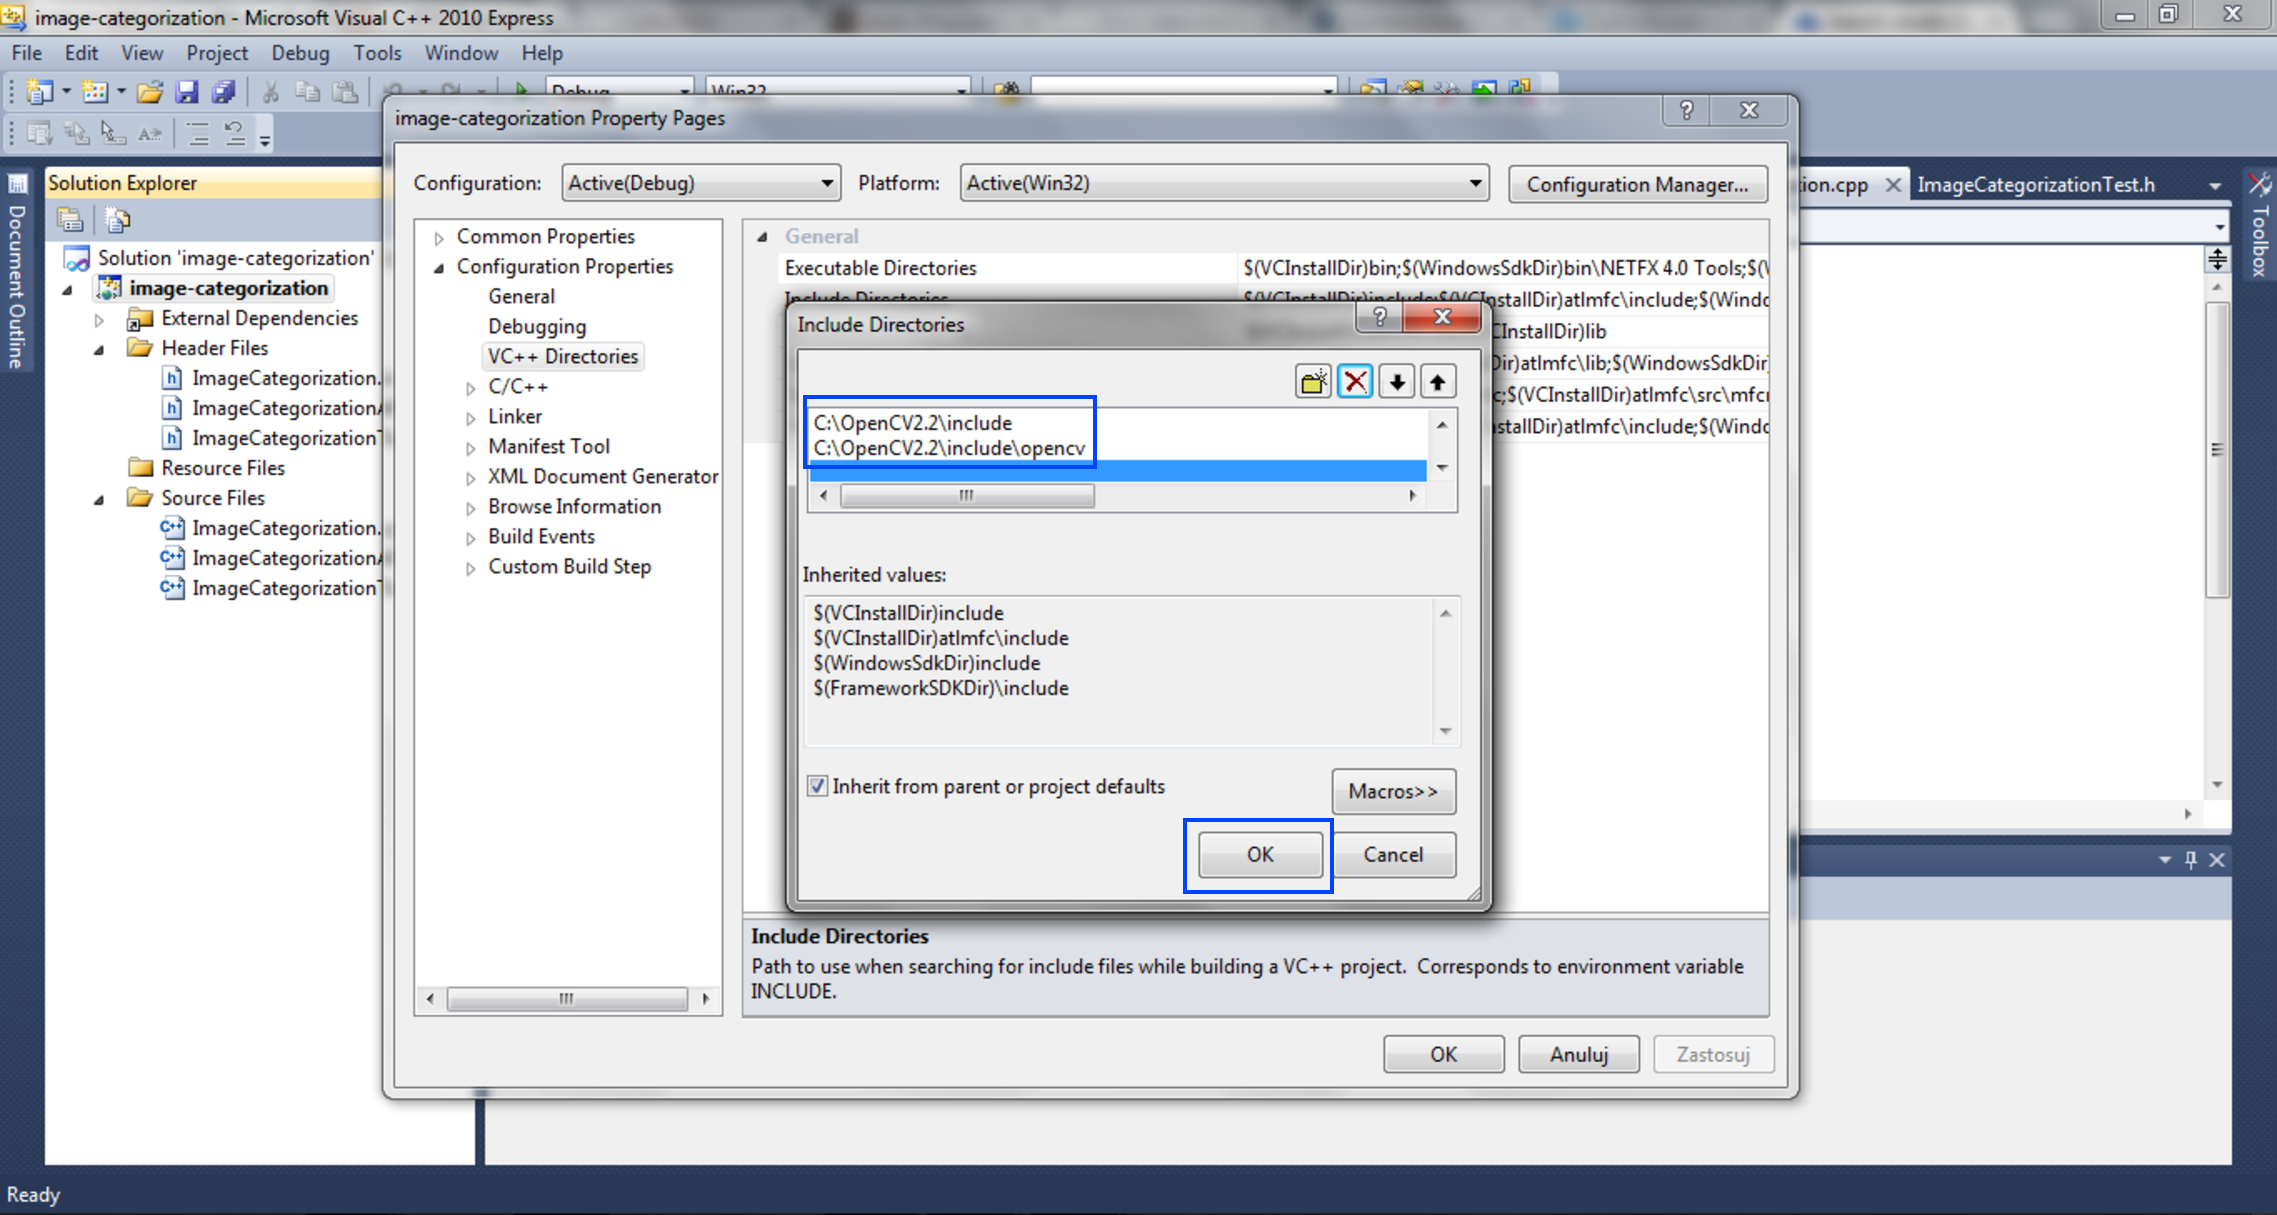
\includegraphics[scale=0.4]{graphics/03_implementacja/ustawienia-include-dirs.pdf}
		\caption{ Ustawienie dołączania katalogów OpenCV }
		\label{fig:ustawienia-include-dirs}
	\end{figure}
	
	\item Pozostając w ustawieniach "VC++ Directories" należy w podobny sposób edytować "Library Directories", dodając ścieżkę \emph{C:\textbackslash OpenCV2.2\textbackslash lib} (rys. \ref{fig:ustawienia-lib-dirs}).
	
	\begin{figure}[h]
		\centering
		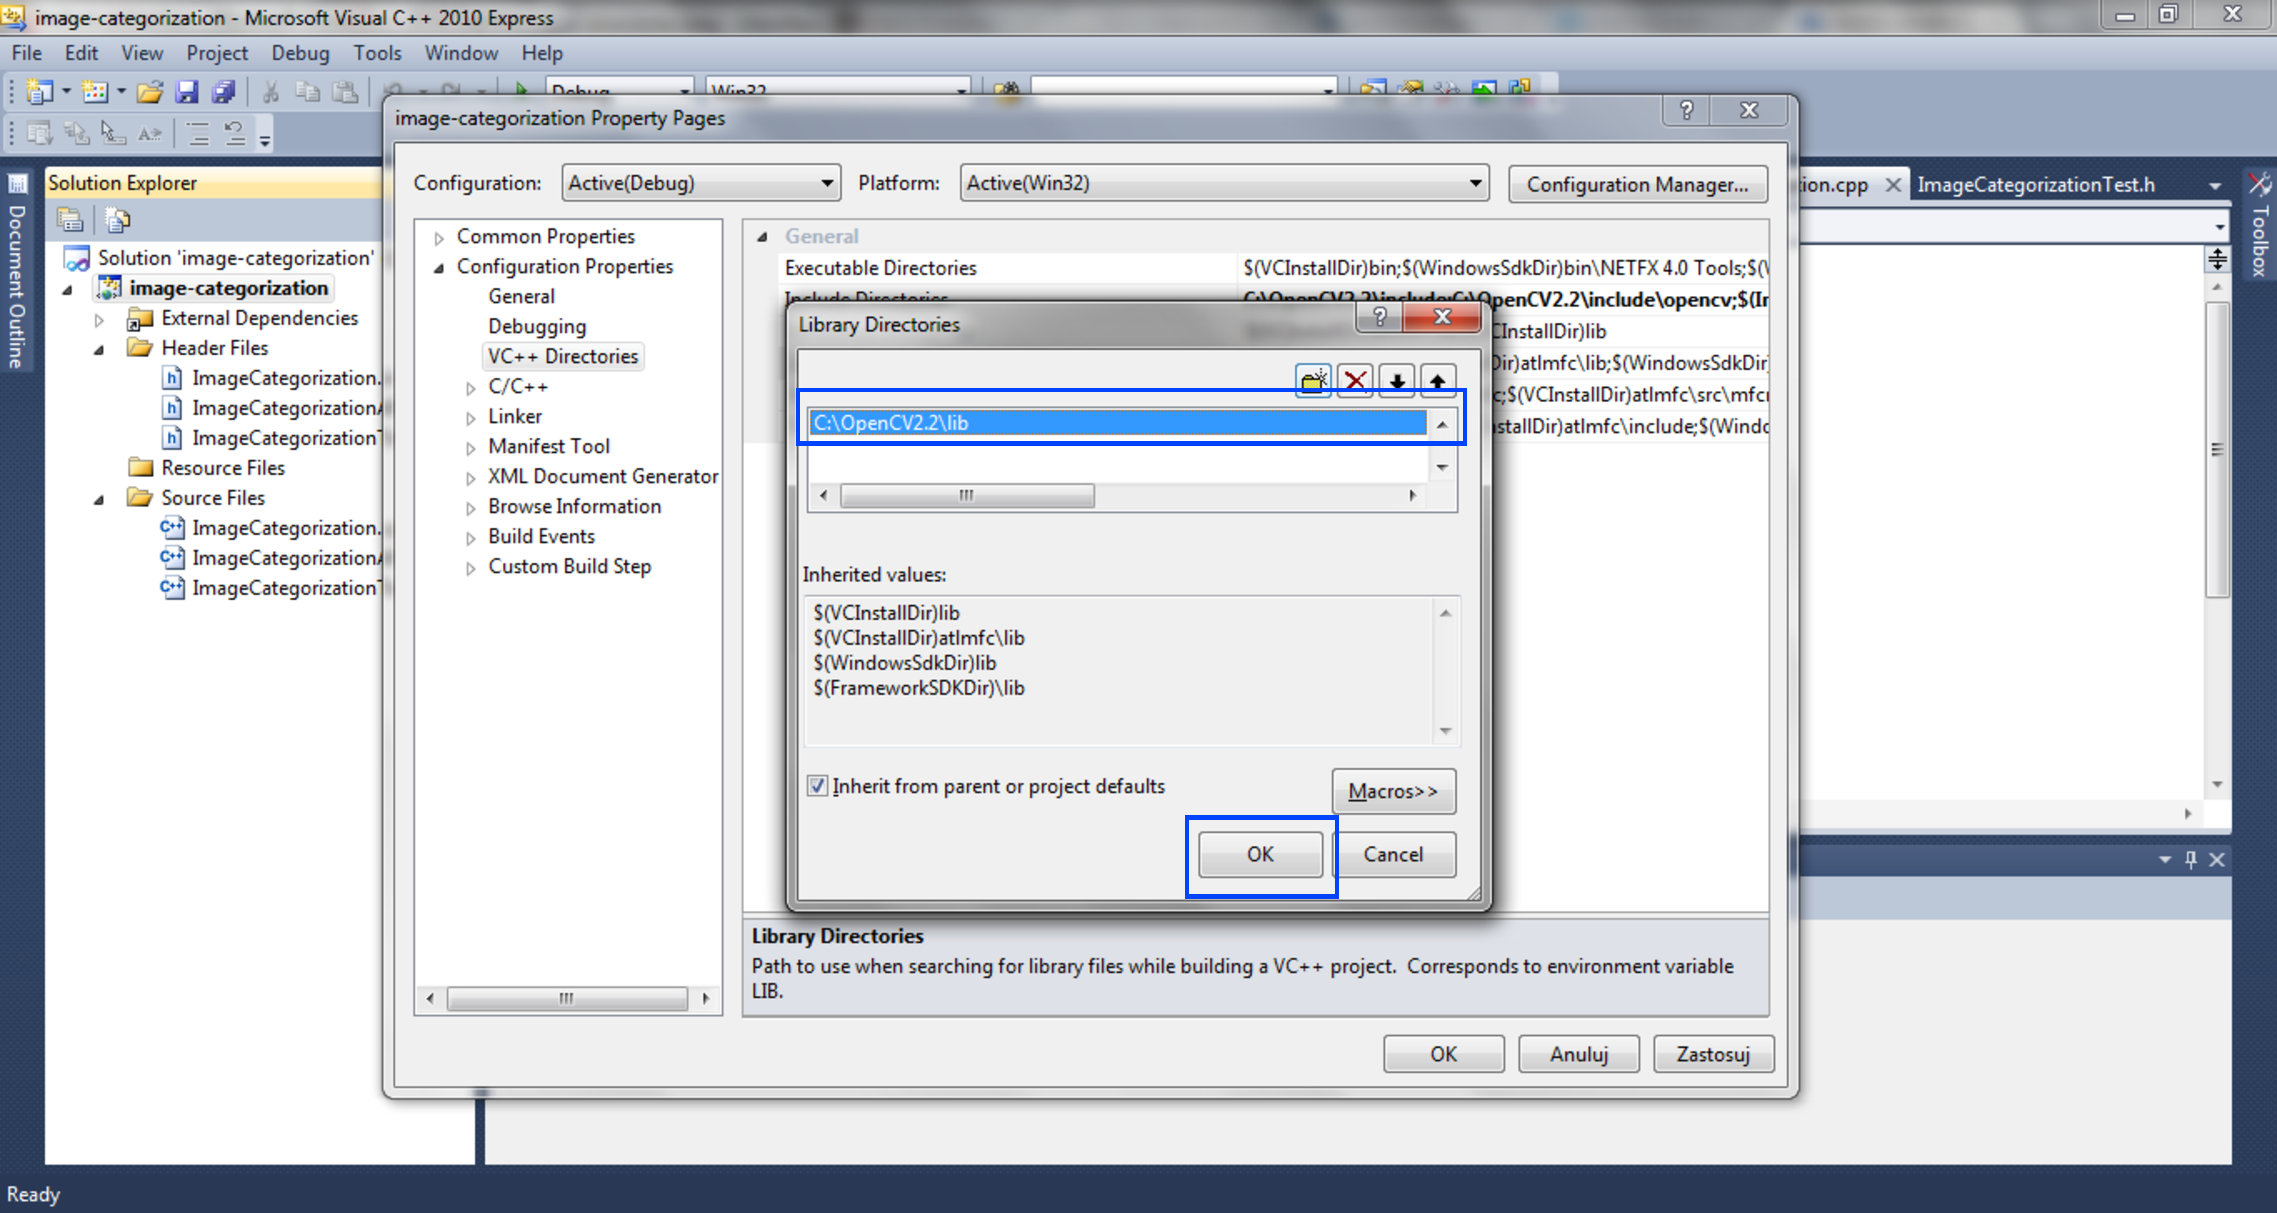
\includegraphics[scale=0.4]{graphics/03_implementacja/ustawienia-lib-dirs.pdf}
		\caption{ Ustawienie dołączania bibliotek OpenCV }
		\label{fig:ustawienia-lib-dirs}
	\end{figure}
	
	\item Następnie należy przejść do ustawień konsolidatora \emph{ang. linker} wybierając z listy opcję "Linker" a następnie "Input" i "Additional Dependencies". W oknie należy umieścić listę potrzebnych bibliotek pakietu OpenCV (rys. \ref{fig:ustawienia-linker}):
	
		\begin{compactitem}
			\item C:\textbackslash OpenCV2.2\textbackslash lib\textbackslash opencv\_core220d.lib
		\item C:\textbackslash OpenCV2.2\textbackslash lib\textbackslash opencv\_highgui220d.lib
		\item C:\textbackslash OpenCV2.2\textbackslash lib\textbackslash opencv\_video220d.lib
		\item C:\textbackslash OpenCV2.2\textbackslash lib\textbackslash opencv\_ml220d.lib
		\item C:\textbackslash OpenCV2.2\textbackslash lib\textbackslash opencv\_legacy220d.lib
		\item C:\textbackslash OpenCV2.2\textbackslash lib\textbackslash opencv\_imgproc220d.lib
		\item C:\textbackslash OpenCV2.2\textbackslash lib\textbackslash opencv\_objdetect220d.lib
		\item C:\textbackslash OpenCV2.2\textbackslash lib\textbackslash opencv\_features2d220d.lib
		\item C:\textbackslash OpenCV2.2\textbackslash lib\textbackslash opencv\_flann220d.lib
		\item C:\textbackslash OpenCV2.2\textbackslash lib\textbackslash opencv\_calib3d220d.lib
		\end{compactitem}
		
		\begin{figure}[h]
			\centering
			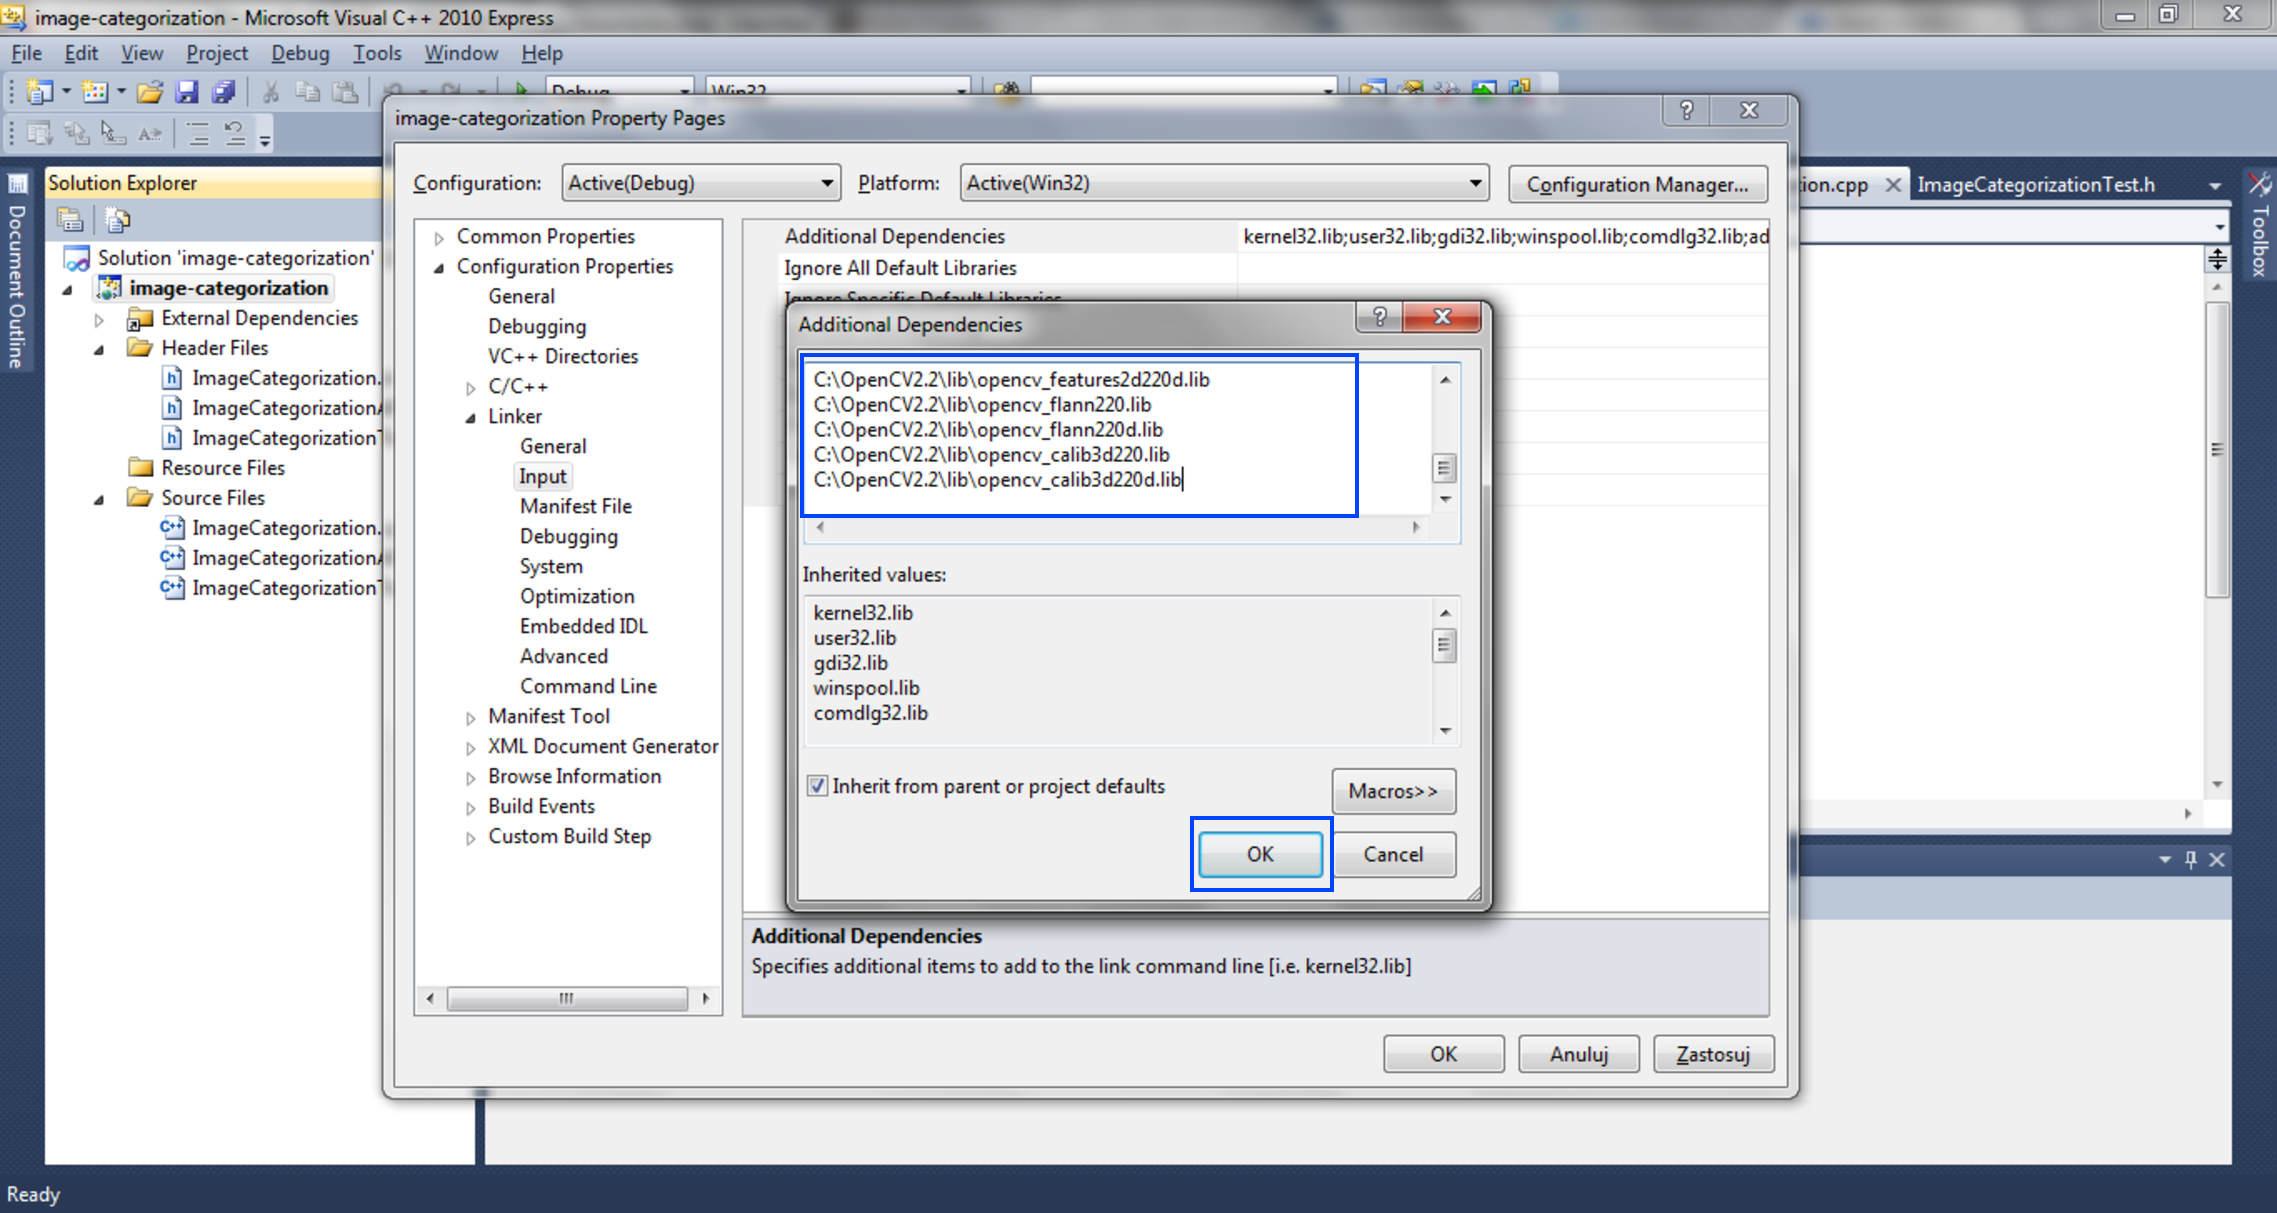
\includegraphics[scale=0.4]{graphics/03_implementacja/ustawienia-linker.pdf}
			\caption{ Ustawienie konsolidatora }
			\label{fig:ustawienia-linker}
		\end{figure}
	
	Po umieszczeniu listy wymaganych bibliotek należy kliknąć przycisk "OK", a następnie wyjść z ustawień projektu klikając ponownie na "OK".
	
	\item Projekt można uruchomić poprzez naciśnięcie przycisku F5 na klawiaturze.
\end{enumerate}

\section{Opis API}

Klasa \emph{ImageCategorizationAPI}\footnote{API - Application Programming Interface; ściśle określony zestaw reguł i ich opisów, w jaki programy komunikują się między sobą.} zawiera następujące metody umożliwiające wykonywanie zadań związanych z kategoryzacją obrazów:

\begin{compactitem}
	\item \texttt{void refreshModel(string path)} -- umożliwia zbudowanie modelu kategoryzacyjnego. Parametr \texttt{path} powinien zawierać ścieżkę do zbioru obrazów służących do zbudowania modelu. Zbiór ten powinien składać się z katalogów, których nazwy odpowiadają kategoriom. W każdym z tych katalogów należy umieścić obrazy służące do uczenia klasyfikatora w podkatalogu \texttt{learn} oraz obrazy służące do testowania klasyfikatora w katalogu \texttt{test}. Przykładowe drzewo katalogów znajduje się na rys. \ref{fig:api-directory-tree}.
	
	\begin{figure}[h]
		\centering
		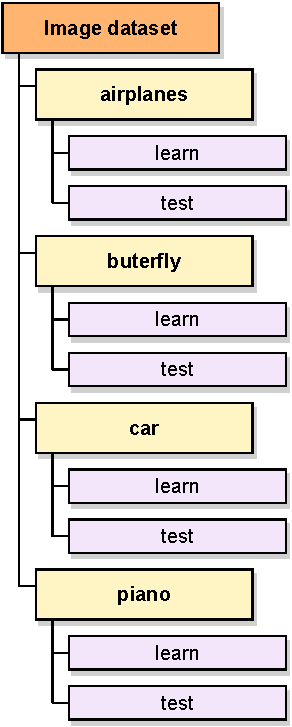
\includegraphics[scale=1.0]{graphics/03_implementacja/api-directory-tree.pdf}
		\caption{ Pryzkładowe drzewo katalogów służące do wytrenowania klasyfikatora }
		\label{fig:api-directory-tree}
	\end{figure}
	
	\item \texttt{string getCategory(string path)} -- zwraca nazwę kategorii przewidzianą przez silnik kategoryzacyjny, np. \emph{airplanes}, \emph{buterfly}. Parametr \texttt{path} powinien być prawidłową ścieżką do obrazu, który chcemy skategoryzować.
\end{compactitem}